\let\negmedspace\undefined
\let\negthickspace\undefined
\documentclass[journal]{IEEEtran}


\setlength{\headheight}{1cm} % Set the height of the header box
\setlength{\headsep}{0mm}     % Set the distance between the header box and the top of the text
 \usepackage[a4paper,margin=10mm, onecolumn]{geometry}
\usepackage{gvv-book}
\usepackage{gvv}
\usepackage{cite}
\usepackage{amsmath,amssymb,amsfonts,amsthm}
\usepackage{algorithmic}
\usepackage{graphicx}
\usepackage{textcomp}
\usepackage{xcolor}
\usepackage{txfonts}
\usepackage{listings}
\usepackage{enumitem}
\usepackage{mathtools}
\usepackage{gensymb}
\usepackage{comment}
\usepackage[breaklinks=true]{hyperref}
\usepackage{tkz-euclide} 
\usepackage{listings}                                       
\def\inputGnumericTable{}                                
\usepackage[latin1]{inputenc}                                
\usepackage{color}                                            
\usepackage{array}                                            
\usepackage{longtable}                                       
\usepackage{calc}                                             
\usepackage{multirow}                                         
\usepackage{hhline}                                           
\usepackage{ifthen}                                           
\usepackage{lscape}
\usepackage{circuitikz}
\tikzstyle{block} = [rectangle, draw, fill=blue!20, 
    text width=4em, text centered, rounded corners, minimum height=3em]
\tikzstyle{sum} = [draw, fill=blue!10, circle, minimum size=1cm, node distance=1.5cm]
\tikzstyle{input} = [coordinate]
\tikzstyle{output} = [coordinate]

\begin{document}

\bibliographystyle{IEEEtran}
\vspace{3cm}

\title{1.6.28}
\author{AI25BTECH11013-Gautham}
 \maketitle
% \newpage
% \bigskip
{\let\newpage\relax\maketitle}

\renewcommand{\thefigure}{\theenumi}
\renewcommand{\thetable}{\theenumi}
\setlength{\intextsep}{10pt} % Space between text and floats


\numberwithin{equation}{enumi}
\numberwithin{figure}{enumi}
\renewcommand{\thetable}{\theenumi}
\textbf{Question}:\\
Show that the points $A(-2\hat{i}+3\hat{j}+5\hat{k}),B(\hat{i}+2\hat{j}+3\hat{k}) and C(7\hat{i}-\hat{k})$are collinear.  \\
\textbf{Solution}:\\
Let the points are $\vec{A}\myvec{-2\\3\\5}$,$\vec{B}\myvec{1\\2\\3}$ and $\vec{C}\myvec{7\\0\\-1}$.
\begin{align}
\vec{B} - \vec{A} = \myvec{1\\2\\3} - \myvec{-2\\3\\5}  \\
\vec{B} - \vec{A} = \myvec{1-(-2)\\2-3\\3-5}  \\
\vec{B} - \vec{A} = \myvec{3\\-1\\-2}  \\
\vec{C} - \vec{A} = \myvec{7\\0\\-1} - \myvec{-2\\3\\5}  \\
\vec{C} - \vec{A} = \myvec{7-(-2)\\0-3\\-1-5}  \\
\vec{C} - \vec{A} = \myvec{9\\-3\\-6}  \\
\end{align}

If $\vec{A}$, $\vec{B}$ and $\vec{C}$ are collinear, then the Rank of matrix $(\vec{B} - \vec{A},\vec{C} - \vec{A})$ should be 1.

\begin{align}
(\vec{B} - \vec{A},\vec{C} - \vec{A}) = \myvec{3&9\\-1&-3\\-2&-6}  \\ 
R_3 \rightarrow (\frac{R_1}{3}\times2) + R_3  \\
R_2 \rightarrow \frac{R_1}{3} + R_2  \\
= \myvec{3&9\\0&0\\0&0}  \\
\end{align}

Since all elements of $R_2$ and $R_3$ are 0, The Rank of matrix $(\vec{B} - \vec{A},\vec{C} - \vec{A})$ is 1.  \\
$\implies$ $\vec{A}$, $\vec{B}$ and $\vec{C}$ are collinear.

\begin{figure}[H]
    \centering
    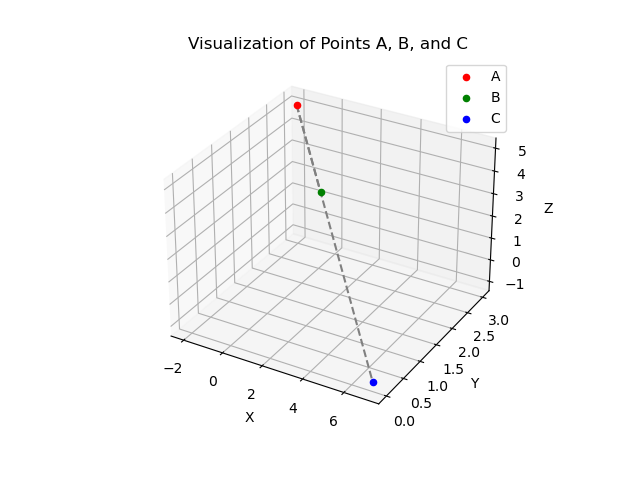
\includegraphics[width=0.8\textwidth]{figs/Fig 1.png}
    \caption{}
    \label{fig:Parallelogram}
\end{figure}

\end{document}
